\section{Join Reordering without statistics}\label{sec:jo}
In prevent section we looked into current state of affair for Join Reordering and why would it not work for Big Data systems. We will like to propose a novel approach in this section to reorder Join just on the basis of table sizes without any elaborate Table or Column Statistics as required by existing approaches.
We have implemented this approach in Apache Spark and will show how our approach gives upto X improvement in TPCDS queries in our empirical evaluation.

\subsection{Heuristics}

Let us look at the assumptions and heuristics used for the approach.

\subsubsection{Assumptions}\label{subsubsec:assumption}:

\begin{itemize}
\item In Star Schema Join, the Dimension table’s primary key will be joined with the Fact table’s foreign key.
\item Cardinality of Fact Table joined with Filtered Dimension table will be less than that of the Fact table.
\item So based on last assumption, it follows that if Fact Join with Filtered Dimension happens earlier in multi-way join, it can benefit later joins.
\end{itemize}

To illustrate assumption above, let's look at this query:
\texttt{select * from fact\_table f join dim1 d1 on f.k1 = d1.pk join dim2 d2 on f.k2 = d2.pk where d2.date = ‘06-10-2019’}. If there is a filter on \texttt{dim2} which is smaller than \texttt{dim1} assumption is it’s join with \texttt{fact\_table} would be smaller than \texttt{fact\_table}. Hence, joining \texttt{fact\_table} with \texttt{dim2} and then with \texttt{dim1} will be beneficial.

\subsubsection{Heuristics for detecting Star schema}
In the lack of statistics, we have to use only table sizes and query structure to determine if a Join is a fact table. We are using following heuristics to determine them:

\begin{itemize}
\item Table involved in all of the joins should be a fact table.
\item At least half of the inner joins in the query should involve the fact table.
\item The ratio of the size of the largest dimensions table to fact table size has to be lesser than a certain threshold.
\item None of the dimensions tables is partitioned.
\end{itemize}

\subsubsection{Constraints for the Join Reorder algorithm}
We will define all the constraints or boundary conditions for the applicability of the algorithm here:

\begin{itemize}
\item \textbf{Star Schema Constraint}: Only Star schema Joins will be considered as assumptions made above are for Star Schema Join only.
\item \textbf{Simple Join Constraint}: Only INNER Joins whose left and right side are comprised of these operators that are deterministic and which do not increase the output size over the input size, other than Join.
\item \textbf{Shuffle Constraint}: For systems having shuffle like Spark or Hive, we reorder only if number of shuffles do not increase due to it. For e.g., consider the following query: \texttt{select * from store\_sales s, item i, web\_sales ws, customer c where s.ss\_item\_sk = i.i\_item\_sk and i.i\_item\_sk = ws.i\_item\_sk and c.c\_customer\_sk = s.ss\_customer\_sk}
\item \textbf{Size Constraint}: Fact table should be atleast $X$ times larger than dimension tables. $X$ is configurable.
\end{itemize}

\subsection{Algorithm}

\begin{algorithm}
\begin{algorithmic}[1]
\STATE  $\Omega$ $\gets$ $R_1$ $\Join$ $R_2$
\IF{$isStarSchemaJoin$($\Omega$) and $isSimpleJoin$($\Omega$) and $obeysShuffleConstraint$($\Omega$)}
    \STATE $type$ $\gets$ $treeType$($\Omega$) \COMMENT{$type$ will be either $left-deep$ or $right-deep$}
    \STATE ($\sigma$, $\delta$[$1$, $\ldots$, $n$]) $\gets$ $extractFactDimensions$($\Omega$)
    \STATE $\theta$[1, $\ldots$, k] $\gets$ $getFilteredDimensions$($\delta$[$1$, $\ldots$, $n$])
    \STATE $\pi$[1, $\ldots$, l] $\gets$ ($\delta$[$1$, $\ldots$, $n$] - $\theta$[1, $\ldots$, k]
    \STATE $\theta$[k+1] $\gets$ $dummyTable1$
    \STATE $dummyDim1$.$size$ $\gets$ $\infty$ 
    \STATE $\pi$[l+1] $\gets$ $dummyTable2$
    \STATE $dummyTable2$.$size$ $\gets$ $-\infty$
    \STATE $i$ $\gets$ 0
    \STATE $j$ $\gets$ 0
    \FOR{$r$ $\gets$ $1$ to $n$} 
        \IF{$\theta$[$i$].size $\geq$ $\pi$[$j$].size}
            \STATE $i$ $\gets$ $i$ $+$ $1$
            \STATE $result$[$r$] $\gets$ $\theta$[$i$]
        \ELSE
            \STATE $j$ $\gets$ $j$ $+$ $1$
            \STATE $result$[$r$] $\gets$ $\pi$[$j$]         
        \ENDIF
    \ENDFOR
    \STATE $\Omega$ $\gets$ $buildJoinTree$($type$, $\sigma$, $result$[$1$, $\ldots$, $n$])
\ENDIF
\RETURN $\Omega$ 
\end{algorithmic}
\label{algorithm}
\caption{Algorithm to Reorder Joins}
\end{algorithm}


Algorithm is presented in \ref{algorithm} where $\Omega$ is assigned to the input Join that needs to be reordered. Following are the summary of steps to reorder them:
\begin{itemize}
\item Check if all constraints are satisfied for a join: \textbf{Star Schema Constraint}, \textbf{Simple Join Constraint}, \textbf{Shuffle Constraint}, \textbf{Size Constraint}.
\item Once it is a star schema, the Join tree can either be \textit{left-deep} or \textit{right-deep}. Obtain the information as we would like to construct reordered join the same way.
\item Extract the Fact table: $\sigma$ and Dimension tables: $ (\delta_1, \delta_2, \ldots, \delta_n)$. For dimension table $\delta_i$, represents  $i^{th}$ dimension table being joined with fact table $\sigma$ from bottom of the Join Tree as shown in Figure \ref{left-deep}. As the tree here would be either \textit{left-deep} or \textit{right-deep} every dimension will have unique $i$ assigned to them. 
\item Split dimensions into two lists: one with selective predicates. $\theta$ and another without it, $\pi$.
\item Sort the list with selective predicates i.e., $\theta$ based on sizes of the dimension tables. Sort the other list i.e., $\pi$ using user provided order.
\item Merge both the list of dimensions by giving user order the preference for tables without selective predicate, whereas for tables with selective predicates giving preference to smaller tables. When comparing top of both the lists, if size of the top table in selective predicate list is smaller than top of other list, choose it otherwise vice-versa. This is in congruence with the Assumption made earlier in sub section \ref{subsubsec:assumption}.
\end{itemize}

\begin{figure}[ht]
\centerline{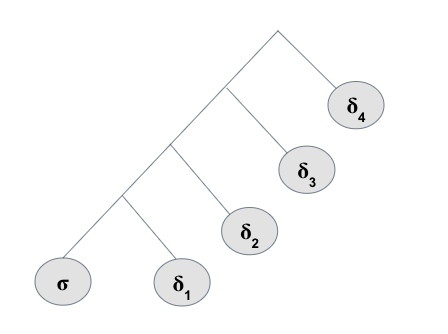
\includegraphics[width=5cm]{fig/left-deep.png}}
\caption{Left-Deep Tree with Fact table $\sigma$ and dimension tables $\delta_i$}
\label{left-deep}
\end{figure}

